\documentclass[11pt,a4paper,titlepage,twoside]{scrartcl}
\usepackage[sfdefault]{FiraSans} % fancy up the font
\usepackage[T1]{fontenc}
\renewcommand*\oldstylenums[1]{{\firaoldstyle #1}}

\usepackage[titletoc]{appendix}
\usepackage{geometry}

\usepackage[english]{babel}
\usepackage[utf8]{inputenc}
\usepackage{enumitem} % referencable enumerations
\usepackage{eurosym}

%\usepackage{biblatex}
%$\addbibresource{references.bib}

\usepackage{tikz}
\usetikzlibrary{calc, positioning, shapes, shapes.geometric, arrows, automata}
\usepackage{adjustbox}

\usepackage{url}
\usepackage{hyperref}

\usepackage{listings}
\usepackage{graphicx}
\usepackage{subcaption}
\usepackage{color}

%\usepackage{natbib}

\AtBeginDocument{\renewcommand\appendixname{Appendix}}



\begin{document}

			%ACTUALLY STARTS FROM HERE, JUST COPIED YOUR SETTINGS FOR PACKAGES

\section*{Early fusion}

\indent	In the second week of the project, we experimented with our setup for Bag of Words framework. We made changes to the method of selecting key points, played a bit with the parameters for the detector/descriptor and number of centroids k for the vocabulary, as well as early fusion of shape and color descriptors in order to produce a better result.
\par	As we already know, we collect key points from features on all images on the training set and then we randomly select predefined number of samples from that pool. For that parameter, we chose 50 000 samples. The issue there might be selecting a lot of points from some images, while other images are not represented in the training process (because the method is to randomly select from all the pool). Moreover, there is no rule to filter already selected points, which means that we can select the same point many times whereas others are left off. We tried to alternate the proposed method in such a way, it no longer selected key point randomly from the whole pool of points. Instead of randomly choosing an image, it iterates through the images and then randomly selects a feature. We believe that with that all the images in the dataset are equally represented, while key points are still selected randomly from the predetermined image in that particular iteration. We are unable to confirm that we improved our results with this technique, as they were really similar to the ones we achieved previously. However, we can say that he computational cost of this small change is insignificant.
\par	Here we also tried to fuse two different feature descriptors in an early fusion fashion – fusion is performed before building the vocabulary. Essentially, it is concatenating the two histograms of both descriptors. We tested  and compared SIFT descriptor, the provided color descriptor and a fusion of both with different parameter for k-means, as shown below on the figure. We also tried fusing the color descriptor with SURF instead of SIFT, but it produced worse results. We observed that SIFT is a lot more effective descriptor than the color descriptor. While parameter k in our test varied, parameters C and number of pixels were fixed and set to 1 and 50000 respectively. We can conclude that early fusion really did help and improved the performances on the given dataset; as seen on the figure below, just with SIFT we got 80 \% accuracy and with early fusion between sift and the color descriptor we achieved the best result of \textbf{82.652 \%}, which is improvement of more than 2.5 \%. We recorded these results with linear SVM kernel for classification and 2000 centroids for k-means. 

\centerline{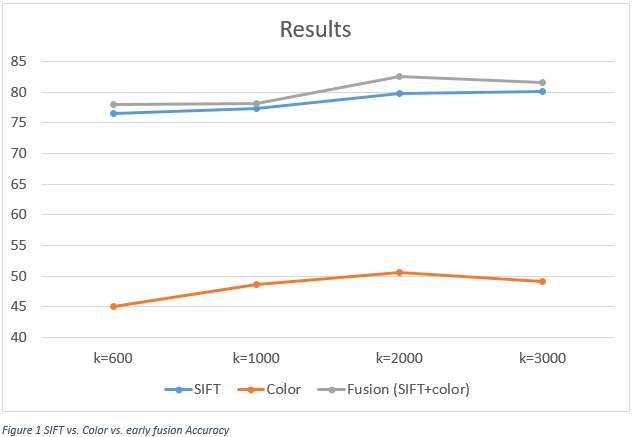
\includegraphics[scale=0.8]{figures/EF.png}}

\par	We should also note that for fusion of 2 different descriptors (in this case color and shape), data whitening (normalization) must be performed before the actual fusion process. That comes from the fact that every descriptor uses different values for describing the features and they are likely to be disproportional, hence the need for normalization.



\section*{Instance retrieval}

\indent    In week 4, we got familiar with the instance retrieval process. We worked on a subset of the ImageNet dataset containing of 2 classes (dog and car). For each class were used 5000 images for training and 150 images for testing. We tested different values for many parameters(detector, descriptor, num. of k-means centroids, global descriptor and query technique). We obtained best results on the following setting: dense sampling for detector, SIFT local descriptor, k=50, Fisher as global descriptor and fast nearest-neighbor for querying. Using those, we recorded top5 accuracy of \textbf{84\%}. That result is highlighted below on dedicated figure, where other results are also shown. 
\par	Using VLAD as a global descriptor, we did not get satisfactory results. With parameters set to k=200 for k-means and fast nearest neighbor querying, dense sampling for detecting features and SIFT for local describing, the top5 performance of the model maxed out at 69\%. We also tested other layouts, like FAST/SIFT and DENSE/SURF for detector/descriptor accordingly, which were less effective. From here on, we used combination of dense sampling and SIFT for local descriptor in the following tests for BoW and Fisher vector as global descriptor.

\centerline{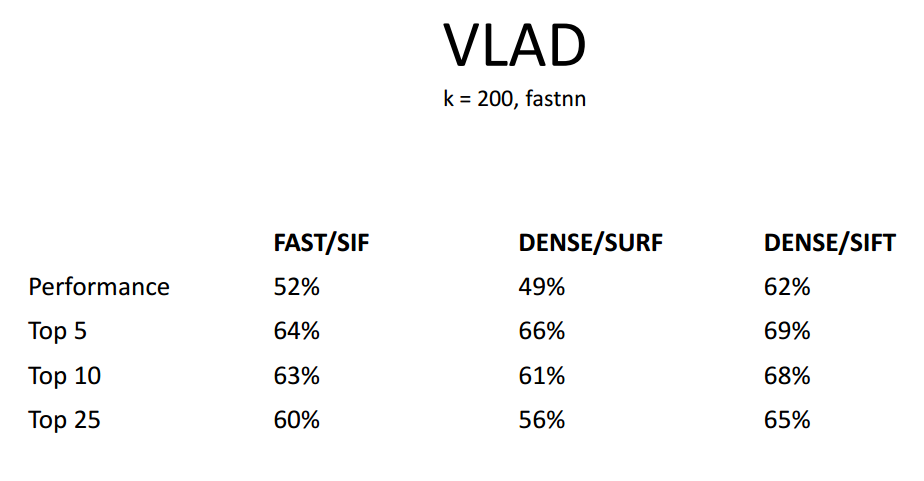
\includegraphics[scale = 0.5]{figures/vlad.png}}

\par Bag of Words as global descriptor performed admirably. We recorded the best performance with vocabulary of size k=500, dense+sift and fast n.n. querying technique, obtaining 79\% top5 accuracy.
\par	Fisher vectors proved to be the best method in our tests. As previously said, the best result we had was 84\% accuracy on top5 with fastnn query. We also tried product quantization (with the default  number of partitions) and locality sensitive hashing on PQ for querying algorithms, which proved to be comparable on smaller vocabulary sizes, but failed to deliver better results on bigger.

\centerline{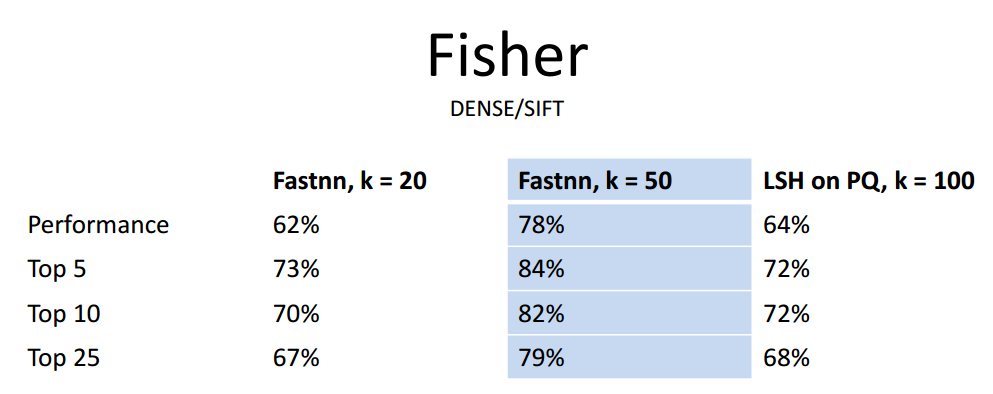
\includegraphics[scale = 0.5]{figures/fish.png}}

\par We are able to conclude that Fisher did perform the best here with vocabulary of only 50 words, but with larger vocabularies it gets too heavy dimensionality-wise as a consequence of the method. Therefore, even 50 words vocabulary with Fisher vector computes slower than 500 words vocabulary on BoW, for example. While dimensionality becomes a big problem for Fisher vectors, also for other techniques we can say that parallelization is a must, since computational cost is heavy on these tasks.

\end{document}
